\documentclass[12pt]{article}

\usepackage{sbc-template}
%\usepackage{titling}
\usepackage{graphicx,url}
\usepackage[utf8]{inputenc}
\usepackage[brazilian]{babel}
\usepackage{booktabs}
\usepackage{amsmath}

\sloppy

\title{Avaliação Comparativa de Algoritmos de Aprendizado de Máquina na Extração do Perfil Comportamental dos Ciclistas Paraenses em 2026  
}



\begin{document}
\address{}

\maketitle

%\begin{abstract}
%  The objective of this study was ......
%\end{abstract}

\begin{resumo} 
  Este artigo propõe uma abordagem híbrida de Aprendizado de Máquina para extrair e validar o perfil comportamental de ciclistas no estado do Pará em 2026. Para processar o banco de dados multivariado contendo variáveis categóricas e numéricas, conduziu-se uma avaliação comparativa de algoritmos não supervisionados, incluindo PAM, K-Means, K-Modes, Modelo Gaussiano, Fuzzy C-Means, CLARA e DBSCAN, utilizando a métrica de dissimilaridade de \textit{Gower}. O particionamento em torno de medoides demonstrou a melhor estabilidade topológica, otimizando a estruturação da amostra em três perfis comportamentais latentes. Posteriormente, a fim de validar preditivamente essa taxonomia e extrair o conhecimento subjacente, aplicou-se o algoritmo supervisionado \textit{Random Forest}. O modelo baseado em árvores de decisão alcançou alta acurácia na reclassificação dos ciclistas e, através da extração do Índice Gini, identificou que features como 'Frequência de Uso', 'Motivo do Deslocamento' e 'Avaliação de Segurança' são os preditores matemáticos mais determinantes na separação dos grupos. Conclui-se que a integração arquitetônica entre modelos de partição, densidade e florestas aleatórias estabelece um framework rigoroso, convertendo dados brutos em inteligência analítica para apoiar políticas públicas de infraestrutura cicloviária.
\end{resumo}


\newpage
\section{Introdução}

A mobilidade urbana sustentável ocupa posição central no debate contemporâneo sobre planejamento urbano, políticas públicas e qualidade de vida nas cidades. Entre os diversos modos de transporte, a bicicleta destaca-se por sua elevada eficiência energética, baixo custo operacional e impactos positivos sobre a saúde individual e coletiva, sendo amplamente reconhecida como instrumento estratégico para a redução de congestionamentos, emissões de poluentes e desigualdades no acesso ao espaço urbano (BANISTER, 2008; PUCHER; BUEHLER, 2012). \vskip0.3cm

No contexto brasileiro, apesar dos avanços recentes na produção de estatísticas públicas sobre mobilidade impulsionados por pesquisas domiciliares, levantamentos amostrais e sistemas administrativos persiste uma lacuna relevante quanto à caracterização sistemática dos usuários de modos ativos, especialmente dos ciclistas urbanos. Grande parte dos estudos nacionais aborda a bicicleta de forma agregada ou secundária, o que limita a compreensão aprofundada de padrões de uso, motivações individuais e barreiras estruturais associadas à mobilidade ciclística (VASCONCELLOS, 2014). \vskip0.3cm

No estado do Pará, essa lacuna é ainda mais pronunciada. A inexistência de bases de dados específicas e atualizadas sobre o perfil do ciclista urbano compromete o planejamento de políticas públicas orientadas por evidências, dificultando a priorização de investimentos em infraestrutura cicloviária, segurança viária e integração modal. Nesse sentido, a realização de pesquisas de campo com coleta de dados primários, padronizados e comparáveis, torna-se fundamental para subsidiar decisões estratégicas no âmbito da gestão pública.


\newpage
\section{Revisão de Literatura}
\subsection{Algoritmos de Aprendizado de Máquina Não Supervisionado}

A tarefa de clusterização consiste em particionar um conjunto de dados em subconjuntos (clusters) maximizando a similaridade intra-grupo e minimizando a similaridade inter-grupos. A seguir, detalham-se os fundamentos matemáticos dos algoritmos avaliados neste estudo.

\subsubsection{Algoritmo K-Means}
O K-Means é um método de partição que busca dividir $N$ observações em $K$ agrupamentos, de forma a minimizar a variância interna de cada grupo. O algoritmo é iterativo e baseia-se no cálculo do centroide (média) das observações \cite{sinaga2020unsupervised}.
\begin{itemize}
    \item \textbf{Função Objetivo (Erro):} Minimiza a Soma dos Erros Quadráticos (SSE - \textit{Sum of Squared Errors}) ou a inércia intra-cluster, dada por:
    $$ J = \sum_{j=1}^{K} \sum_{x_i \in C_j} ||x_i - \mu_j||^2 $$
    onde $\mu_j$ é o centroide do cluster $C_j$ e $x_i$ é o ponto de dado.
    \item \textbf{Métrica de Distância:} Utiliza fundamentalmente a Distância Euclidiana, o que o torna sensível a \textit{outliers} e inadequado matematicamente para variáveis estritamente categóricas.
    \item \textbf{Literatura Recente:} Trabalhos recentes como o de Ahmed et al. (2020) \cite{ahmed2020k} discutem otimizações heurísticas do K-Means para lidar com convergências locais em grandes volumes de dados.
\end{itemize}

\subsubsection{Algoritmo K-Modes}
Uma extensão do K-Means desenvolvida especificamente para lidar com dados categóricos. Em vez de calcular a média euclidiana, o algoritmo utiliza a moda estadística, substituindo o centroide pelo "modo" do grupo \cite{huang1998extensions}.
\begin{itemize}
    \item \textbf{Função Objetivo (Erro):} Minimiza o custo total baseado em incompatibilidades, expresso por:
    $$ J = \sum_{j=1}^{K} \sum_{x_i \in C_j} d_{mm}(x_i, Q_j) $$
    onde $Q_j$ é o modo do cluster e $d_{mm}$ é a medida de dissimilaridade.
    \item \textbf{Métrica de Distância:} Utiliza a Distância de \textit{Simple Matching} (Hamming). A distância é $0$ se os atributos categóricos forem iguais e $1$ se forem diferentes.
    \item \textbf{Literatura Recente:} Cao et al. (2021) \cite{cao2021kmodes} propõem métodos modernos de inicialização para o K-Modes visando melhorar a estabilidade da convergência em dados de \textit{survey}.
\end{itemize}

\subsubsection{Modelo Gaussiano (Gaussian Mixture Model - GMM)}
O GMM é um modelo probabilístico que assume que os dados são gerados por uma mistura de um número finito de distribuições normais (Gaussianas) com parâmetros desconhecidos. Diferente dos métodos de partição rígida, o GMM oferece uma clusterização probabilística \cite{scrucca2016mclust}.
\begin{itemize}
    \item \textbf{Função Objetivo (Erro):} O modelo não minimiza uma distância espacial, mas maximiza a função de \textit{Log-Likelihood} (Verossimilhança) através do algoritmo \textit{Expectation-Maximization} (EM):
    $$ \ln p(X|\pi, \mu, \Sigma) = \sum_{i=1}^{N} \ln \left( \sum_{k=1}^{K} \pi_k \mathcal{N}(x_i | \mu_k, \Sigma_k) \right) $$
    \item \textbf{Métrica de Distância:} Implicitamente, utiliza a Distância de Mahalanobis, pois a covariância $\Sigma_k$ modela a forma elíptica da distribuição.
    \item \textbf{Literatura Recente:} O pacote \texttt{mclust} no R, amplamente detalhado por Scrucca et al. (2023) \cite{scrucca2023mclust}, tornou-se o padrão-ouro para a seleção automática do número de clusters $K$ usando o Critério de Informação Bayesiano (BIC).
\end{itemize}

\subsubsection{Algoritmo Fuzzy C-Means (FCM)}
Diferente do agrupamento rígido (\textit{hard clustering}), o FCM baseia-se na lógica \textit{Fuzzy}, permitindo que uma mesma observação pertença a múltiplos clusters simultaneamente, com diferentes graus de pertinência variando de $0$ a $1$ \cite{bezdek1981pattern}.
\begin{itemize}
    \item \textbf{Função Objetivo (Erro):} Minimiza a função objetiva ponderada pelo grau de pertinência:
    $$ J_m = \sum_{i=1}^{N} \sum_{j=1}^{C} u_{ij}^m ||x_i - c_j||^2 $$
    onde $u_{ij}$ é o grau de pertinência do dado $x_i$ ao cluster $c_j$, e $m$ é o coeficiente de \textit{fuzziness} (geralmente $m=2$).
    \item \textbf{Métrica de Distância:} Tradicionalmente Euclidiana, embora possa ser adaptada.
    \item \textbf{Literatura Recente:} Nayak et al. (2020) \cite{nayak2020fuzzy} aplicam o FCM em mineração de dados complexos, ressaltando a sua capacidade superior no mapeamento de transições comportamentais ou limites topológicos sobrepostos.
\end{itemize}

\subsubsection{Algoritmo PAM (Partitioning Around Medoids)}
O PAM é uma alternativa robusta ao K-Means. Em vez de calcular a média teórica de um grupo, o algoritmo elege um ponto de dado real existente no banco (o medoide) como o centro de referência do cluster \cite{kaufman1990finding}.
\begin{itemize}
    \item \textbf{Função Objetivo (Erro):} Minimiza a soma absoluta das dissimilaridades entre todos os pontos de um cluster e o seu medoide correspondente:
    $$ J = \sum_{j=1}^{K} \sum_{x_i \in C_j} d(x_i, m_j) $$
    onde $m_j$ é o medoide do cluster $j$.
    \item \textbf{Métrica de Distância:} Altamente flexível. Em dados mistos, adota-se a Distância de \textit{Gower}, que normaliza variáveis numéricas pelo seu alcance e variáveis categóricas via índice de correspondência simples.
    \item \textbf{Literatura Recente:} Schubert e Rousseeuw (2019) \cite{schubert2019faster} otimizaram matematicamente o algoritmo através do \textit{FasterPAM}, permitindo sua aplicação em \textit{Big Data} com complexidade de tempo linear.
\end{itemize}

\subsubsection{Algoritmo CLARA (Clustering Large Applications)}
O CLARA é uma extensão do PAM projetada para contornar a alta complexidade computacional associada ao cálculo da matriz de distância par-a-par em bancos de dados massivos.
\begin{itemize}
    \item \textbf{Conceito e Erro:} Em vez de buscar medoides na população total, o CLARA extrai diversas amostras aleatórias, aplica o PAM tradicional em cada subamostra e retorna a solução que obteve a menor distância média de todos os dados do banco original em relação aos medoides amostrais.
    \item \textbf{Métrica de Distância:} Frequentemente implementado usando as distâncias Euclidiana ou de Manhattan.
    \item \textbf{Literatura Recente:} Pesquisas em mineração de dados em larga escala frequentemente comparam o CLARA com o K-Means devido à sua escalabilidade mantendo a robustez aos \textit{outliers} \cite{schubert2021clara}.
\end{itemize}

\subsubsection{Algoritmo DBSCAN (Densidade)}
O \textit{Density-Based Spatial Clustering of Applications with Noise} não parte do princípio da partição em torno de um centro, mas constrói clusters procurando regiões de alta densidade no hiper-espaço e isolando pontos em áreas ralas como ruído (ruído topológico) \cite{ester1996density}.
\begin{itemize}
    \item \textbf{Função Matemática:} É definido por dois parâmetros: o raio de vizinhança ($\epsilon$) e o número mínimo de pontos ($\textit{minPts}$). Um ponto $p$ é considerado central se houver pelo menos $\textit{minPts}$ pontos na sua $\epsilon$-vizinhança.
    \item \textbf{Métrica de Distância:} Pode utilizar matrizes personalizadas como Euclidiana, Manhattan ou, no contexto categórico, a métrica de \textit{Gower}.
    \item \textbf{Literatura Recente:} Hahsler et al. (2019) \cite{hahsler2019dbscan} apresentam implementações modernas em R que potencializam algoritmos baseados em densidade para identificação precisa de anomalias em transportes.
\end{itemize}

\subsection{Algoritmo Supervisionado: Random Forest}
A \textit{Random Forest} é um método de \textit{Ensemble Learning} que constrói uma "floresta" composta por dezenas ou centenas de Árvores de Decisão independentes, treinadas a partir de subconjuntos aleatórios de dados (técnica de \textit{Bagging}) e de \textit{features} \cite{breiman2001random}. Neste estudo, sua função primária é validar a precisão dos clusters e ranquear a importância das variáveis por meio de Inteligência Artificial Explicável (XAI).
\begin{itemize}
    \item \textbf{Critério de Divisão (Erro):} Na classificação, o modelo avalia os cortes nos nós utilizando o Índice de Impureza de \textit{Gini}, que mede a probabilidade de um elemento selecionado aleatoriamente ser classificado incorretamente:
    $$ G = 1 - \sum_{i=1}^{C} p_i^2 $$
    onde $p_i$ é a proporção da classe $i$ no nó. A queda média dessa impureza (\textit{Mean Decrease Gini}) quantifica o poder discriminatório de cada pergunta do questionário.
    \item \textbf{Literatura Recente:} Biau e Scornet (2016) \cite{biau2016random} consolidam as bases teóricas do algoritmo, enquanto a literatura moderna explora a extração de Valores SHAP para a explicabilidade avançada do modelo.
\end{itemize}






\section{Material e Métodos}
\subsection{Localização e Levantamento dos Dados}

A população-alvo da pesquisa é composta por indivíduos com idade igual ou superior a 12
anos que utilizam a bicicleta como meio de transporte ao menos uma vez por semana em
ambiente urbano. Incluem-se usuários que estejam, no momento da abordagem, utilizando,
estacionando ou conduzindo a bicicleta a pé. \vskip0.3cm

Do ponto de vista conceitual, distingue-se a população-alvo conjunto teórico sobre o qual se
deseja inferir da população efetivamente investigada, limitada pelas condições operacionais
da coleta. A inexistência de cadastros formais ou registros administrativos que identifiquem
usuários de bicicleta inviabiliza a adoção de métodos clássicos de amostragem probabilística,
como amostragem aleatória simples ou estratificada (Lohr, 2019). \vskip0.3cm

Diante dessas limitações, será adotada uma estratégia de amostragem não probabilística por
interceptação em pontos estratégicos da malha urbana, tais como vias arteriais, ciclovias, áreas
comerciais, polos geradores de viagens e equipamentos públicos. Essa abordagem é amplamente utilizada em pesquisas de mobilidade ativa e transporte urbano, especialmente quando o universo populacional é desconhecido ou de difícil mensuração (Stopher \& Jones, 2003). \vskip0.3cm

O tamanho da amostra será definido a partir de estimativas do universo de ciclistas fornecidas por fontes secundárias, como o Sistema de Informações da Mobilidade Urbana da Associação Nacional de Transportes Públicos (ANTP), combinadas com critérios operacionais e recursos disponíveis. Embora não permita inferência estatística estrita para toda a população, essa abordagem possibilita a construção de diagnósticos robustos e indicativos para formulação de políticas públicas. \vskip0.3cm

Adota-se, para fins operacionais, um erro amostral máximo de 10\%, compatível com levantamentos exploratórios em populações de difícil mensuração, conforme práticas consolidadas em pesquisas de mobilidade urbana. \vskip0.3cm

\section{Instrumento de Pesquisa}

O instrumento de coleta consiste em um questionário estruturado, composto predominantemente por perguntas fechadas, elaborado com base em referenciais metodológicos de pesquisas nacionais e internacionais sobre mobilidade ativa e comportamento do ciclista urbano (HEINEN; VAN WEE; MAAT, 2010; PUCHER; BUEHLER, 2017)


%------------------------------------------------------------------%
\section{Resultados e Discussão}
\subsection{Análise Descritiva de Dados}



\begin{table}[htbp]
\centering
\caption{Perfil Estatístico e Comportamental dos Ciclistas Paraenses por Grupo (2026)}
\label{tab:perfil_grupos}
\resizebox{\textwidth}{!}{%
\begin{tabular}{@{}l|c|c|c@{}}
\hline \hline
\textbf{Características} & \textbf{Grupo 1} & \textbf{Grupo 2} & \textbf{Grupo 3} \\ 
\hline \hline
Município             & Marabá (12.9\%) & Castanhal (18.4\%) & Marabá (26.8\%) \\
Tipo de Bicicleta     & Convencional (98.6\%) & Convencional (84.4\%) & Convencional (91.9\%) \\
Gênero                & Masculino (67.1\%) & Feminino (69.3\%) & Feminino (75.8\%) \\
Faixa Etária          & De 30 a 49 anos (34.6\%) & De 19 a 29 anos (58.7\%) & De 30 a 49 anos (41.4\%) \\
Raça                  & Parda (9.4\%) & Parda (67.6\%) & Parda (57.1\%) \\
Escolaridade          & Ensino médio (50\%) & Ensino médio (72.1\%) & Ensino superior (53\%) \\
Ocupação Principal    & Trab. informal (28.3\%) & Trab. formal (45.3\%) & Trab. formal (46.5\%) \\
Renda Mensal          & Até 1 salário mínimo (56.3\%) & De 1 a 3 sal. mínimos (49.2\%) & De 1 a 3 sal. mínimos (54\%) \\
Frequência de Uso     & Todos os dias (56\%) & Todos os dias (38.5\%) & De 1 a 2 dias/semana (77.3\%) \\
Tempo Médio (Uso)     & Até 20 minutos (32.6\%) & Até 20 minutos (39.7\%) & Até 10 minutos (50.5\%) \\
Tempo como Transporte & Acima de 6 anos (70.9\%) & Acima de 6 anos (32.4\%) & Menos de 6 meses (39.4\%) \\
Destino Principal     & Trabalho (46.6\%) & Trabalho (41.9\%) & Lazer ou ativ. sociais (42.4\%) \\
Maior Motivação       & Economia financeira (52\%) & Economia financeira (38.5\%) & Benefícios à saúde (35.9\%) \\
Sofreu Acidente(s)    & Não (74.9\%) & Não (78.8\%) & Não (85.4\%) \\
Bicicleta Furtada     & Não (70.3\%) & Não (75.4\%) & Não (74.2\%) \\
Risco ao Pedalar      & Vel. Veículos / Falta infra. (46.3\%) & Vel. Veículos / Falta infra. (45.8\%) & Falta infra. / Iluminação (23.2\%) \\
Usa + a Bike Pós-COVID   & Sim (54.6\%) & Sim (50.3\%) & Não (65.2\%) \\
Governo Incentiva Uso    & Não (79.7\%) & Parcialmente (44.7\%) & Não (84.8\%) \\ \bottomrule
\end{tabular}%
}
\end{table}


\subsection{Validação Cruzada: PAM versus Algoritmos Alternativos}

Para atestar a estabilidade estrutural e a validade topológica dos três perfis descobertos, o particionamento oficial gerado pelo algoritmo PAM (com métrica de Gower) foi submetido a uma validação cruzada contra as partições geradas por K-Means, K-Modes, Modelo Gaussiano (GMM) e Fuzzy C-Means. A análise das matrizes de concordância revela o comportamento de cada heurística perante a complexidade dos dados categóricos de mobilidade.

\subsubsection{O Colapso do K-Means em Dados Categóricos}
A comparação entre PAM e K-Means evidenciou a inadequação de métricas euclidianas clássicas para dados sociocomportamentais. O algoritmo K-Means sofreu um colapso de variância, alocando 77\% de toda a amostra (557 dos 727 ciclistas) num único super-grupo espúrio, denominado Grupo Y. 
\begin{itemize}
    \item Este super-grupo absorveu quase a totalidade dos três perfis do PAM (274 do Perfil 1, 133 do Perfil 2 e 150 do Perfil 3).
    \item A incapacidade do K-Means em calcular médias aritméticas válidas para respostas qualitativas resultou numa severa aglomeração (\textit{crowding problem}), impossibilitando a extração de qualquer padrão comportamental acionável para políticas públicas.
\end{itemize}

\subsubsection{Convergência Parcial com o K-Modes}
Ao contrário do K-Means, o K-Modes (desenhado para dados categóricos) demonstrou forte concordância topológica com os perfis extremos do PAM, validando a sua existência:
\begin{itemize}
    \item \textbf{Alinhamento do Perfil Principal:} O Perfil 1 do PAM obteve forte correspondência com o Perfil A do K-Modes, partilhando 205 ciclistas (28\% da amostra global).
    \item \textbf{Alinhamento do Perfil Específico:} O Perfil 3 do PAM alinhou-se de forma substancial com o Perfil B do K-Modes (164 ciclistas partilhados).
    \item \textbf{Divergência no Perfil Intermédio:} O Perfil 2 apresentou alta fragmentação, distribuindo-se de forma quase equitativa entre os três grupos do K-Modes. Isto sugere que o K-Modes, ao basear-se apenas na moda estatística (\textit{Simple Matching}), perde sensibilidade analítica nos grupos de transição, onde a métrica de Gower (utilizada pelo PAM) é mais eficaz ao ponderar semelhanças parciais.
\end{itemize}

\subsubsection{A Sobre-segmentação do Modelo Gaussiano (GMM)}
O modelo probabilístico Gaussiano (GMM) utilizou o Critério de Informação Bayesiano (BIC) para definir o número ideal de agrupamentos, convergindo autonomamente para $K=4$. A introdução deste quarto grupo revela uma tentativa do algoritmo de acomodar a variância esparsa dos dados:
\begin{itemize}
    \item O Perfil 1 (PAM) encontrou o seu núcleo no Grupo 2 do GMM (209 ciclistas).
    \item O Perfil 3 (PAM) consolidou-se solidamente no Grupo 3 do GMM (153 ciclistas).
    \item A fragmentação severa ocorreu novamente no Perfil 2, que se diluiu por todos os quatro clusters gaussianos. A criação do Grupo 4 (GMM), com 82 ciclistas, capta micro-comportamentos que o PAM optou por aglutinar para manter a parcimónia analítica. No contexto de planeamento urbano, um modelo mais limpo ($K=3$) é preferível a um modelo sobre-segmentado.
\end{itemize}

\subsubsection{A Diluição das Fronteiras no Fuzzy C-Means}
A aplicação da lógica difusa (\textit{Fuzzy C-Means}) com os dados forçados a um formato numérico replicou parcialmente a falha do K-Means, embora com menor agressividade.
\begin{itemize}
    \item Ocorreu uma forte polarização binária: o Grupo Beta absorveu 43\% da amostra (316 ciclistas) e o Grupo Gama absorveu 38\% (275 ciclistas), deixando o Grupo Alpha esvaziado (19\%).
    \item O Perfil 1 do PAM foi drasticamente fraturado entre o Grupo Beta (181) e o Grupo Gama (104).
    \item O coeficiente de pertinência difusa (\textit{fuzziness}) não conseguiu lidar com a sobreposição categórica, resultando num esbatimento das fronteiras comportamentais que o PAM conseguiu delinear de forma muito mais nítida e interpretável através do isolamento de medoides reais.
\end{itemize}
















\begin{figure}
    \centering
    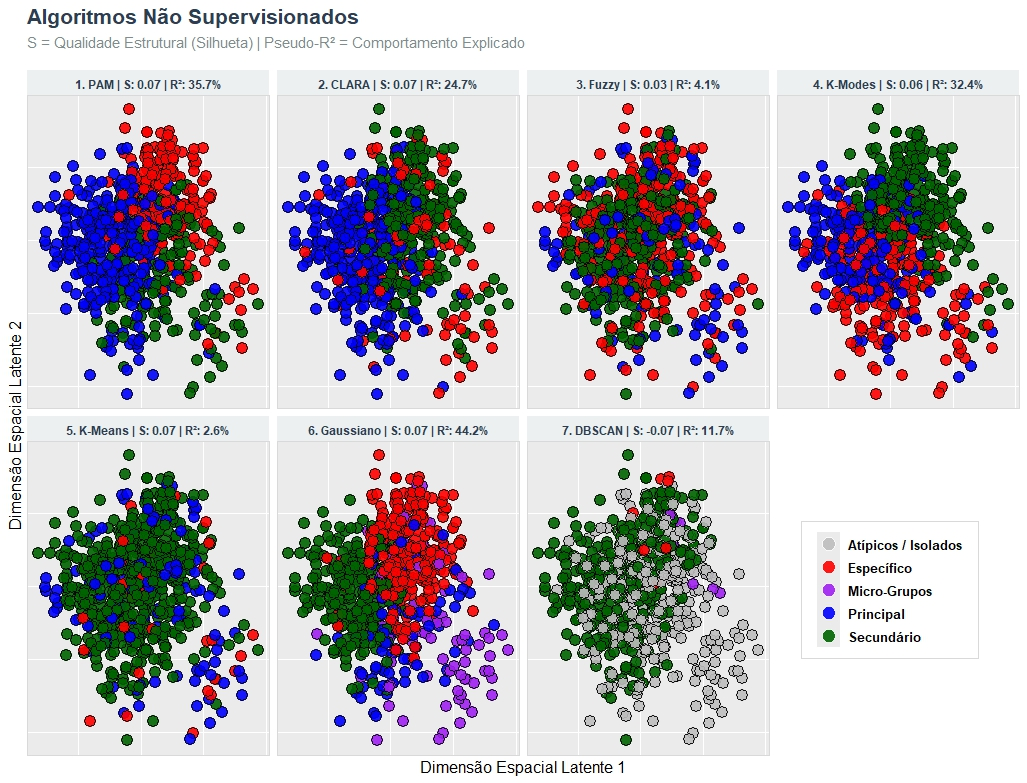
\includegraphics[width=1\linewidth]{Rplot02.jpeg}
    \caption{Algoritmos de Aprendizado de Máquina Não Supervisionados para amostra de Ciclista no Pará em 2026.}
    \label{fig:placeholder}
\end{figure}



\newpage
\section{Considerações Finais}

%Este estudo demonstrou a viabilidade e a superioridade de abordagens híbridas de Aprendizado de Máquina para a extração de conhecimento em bases de dados de mobilidade urbana. A avaliação comparativa atestou que algoritmos de partição baseados em medoides (PAM), quando acoplados a métricas de dissimilaridade adequadas (\textit{Gower}), superam métodos euclidianos clássicos (K-Means) e de densidade (DBSCAN) na estruturação de dados comportamentais esparsos. \vskip0.3cm

%A taxonomia descoberta revela que o ciclista paraense em 2026 não constitui um grupo homogêneo, mas divide-se entre usuários utilitários históricos, predominantemente vulneráveis do ponto de vista socioeconômico, e um novo contingente de usuárias focadas em saúde e lazer. Esta heterogeneidade exige que o Estado abandone soluções genéricas de infraestrutura.  \vskip0.3cm

%Como trabalhos futuros, sugere-se a aplicação da explicabilidade de modelos (\textit{Explainable AI}), como Valores SHAP derivados da \textit{Random Forest}, para quantificar de forma isolada o peso probabilístico de variáveis geográficas na determinação de cada cluster, ampliando o arcabouço de apoio à tomada de decisão no planejamento viário.

\bibliographystyle{sbc}
\bibliography{sbc-template} 

\end{document}